%\documentclass[honours,12pt,twoside]{unswthesis}

\usepackage{afterpage}
\usepackage{amsfonts}
\usepackage{amsmath}
\usepackage{amssymb}
\usepackage{amsthm}
\usepackage[english]{babel}
\usepackage{graphicx}
\usepackage{natbib}
\usepackage[utf8]{inputenc}
\usepackage{latexsym}
\usepackage{url}
\usepackage{todonotes}
\usepackage{tikz}
\usepackage{pdfpages}
\usetikzlibrary{arrows}
\usepackage{float}

\usepackage{booktabs}
\renewcommand{\arraystretch}{1.2}


%%%%%%%%%%%%%%%%%%%%%%%%%%%%%%%%%%%%%%%%%%%%%%%%%%%%%%%%%%%%%%%%%
%
%  The following are some simple LaTeX macros to give some
%  commonly used letters in funny fonts. You may need more or less of
%  these
%
\newcommand{\R}{\mathbb{R}}
\newcommand{\Q}{\mathbb{Q}}
\newcommand{\C}{\mathbb{C}}
\newcommand{\N}{\mathbb{N}}
\newcommand{\F}{\mathbb{F}}
\newcommand{\PP}{\mathbb{P}}
\newcommand{\T}{\mathbb{T}}
\newcommand{\Z}{\mathbb{Z}}
\newcommand{\B}{\mathfrak{B}}
\newcommand{\BB}{\mathcal{B}}
\newcommand{\M}{\mathfrak{M}}
\newcommand{\X}{\mathfrak{X}}
\newcommand{\Y}{\mathfrak{Y}}
\newcommand{\CC}{\mathcal{C}}
\newcommand{\E}{\mathbb{E}}
\newcommand{\cP}{\mathcal{P}}
\newcommand{\cS}{\mathcal{S}}
\newcommand{\A}{\mathcal{A}}
\newcommand{\ZZ}{\mathcal{Z}}

%%%%%%%%%%%%%%%%%%%%%%%%%%%%%%%%%%%%%%%%%%%%%%%%%%%%%%%%%%%%%%%%%%%%%
%
% The following are much more esoteric commands that I have left in
% so that this file still processes. Use or delete as you see fit
%
\newcommand{\bv}[1]{\mbox{BV($#1$)}}
\newcommand{\comb}[2]{\left(\!\!\!\begin{array}{c}#1\\#2\end{array}\!\!\!\right)
}
\newcommand{\Lat}{{\rm Lat}}
\newcommand{\var}{\mathop{\rm var}}
\newcommand{\Pt}{{\mathcal P}}
\def\tr(#1){{\rm trace}(#1)}
\def\Exp(#1){{\mathbb E}(#1)}
\def\Exps(#1){{\mathbb E}\sparen(#1)}
\newcommand{\floor}[1]{\left\lfloor #1 \right\rfloor}
\newcommand{\ceil}[1]{\left\lceil #1 \right\rceil}
\newcommand{\hatt}[1]{\widehat #1}
\newcommand{\modeq}[3]{#1 \equiv #2 \,(\text{mod}\, #3)}
\newcommand{\rmod}{\,\mathrm{mod}\,}
\newcommand{\p}{\hphantom{+}}
\newcommand{\vect}[1]{\mbox{\boldmath $ #1 $}}
\newcommand{\reff}[2]{\ref{#1}.\ref{#2}}
\newcommand{\psum}[2]{\sum_{#1}^{#2}\!\!\!'\,\,}
\newcommand{\bin}[2]{\left( \begin{array}{@{}c@{}}
				#1 \\ #2
			\end{array}\right)	}
%
%  Macros - some of these are in plain TeX (gasp!)
%
\newcommand{\be}{($\beta$)}
\newcommand{\eqp}{\mathrel{{=}_p}}
\newcommand{\ltp}{\mathrel{{\prec}_p}}
\newcommand{\lep}{\mathrel{{\preceq}_p}}
\def\brack#1{\left \{ #1 \right \}}
\def\bul{$\bullet$\ }
\def\cl{{\rm cl}}
\let\del=\partial
\def\enditem{\par\smallskip\noindent}
\def\implies{\Rightarrow}
\def\inpr#1,#2{\t \hbox{\langle #1 , #2 \rangle} \t}
\def\ip<#1,#2>{\langle #1,#2 \rangle}
\def\lp{\ell^p}
\def\maxb#1{\max \brack{#1}}
\def\minb#1{\min \brack{#1}}
\def\mod#1{\left \vert #1 \right \vert}
\def\norm#1{\left \Vert #1 \right \Vert}
\def\paren(#1){\left( #1 \right)}
\def\qed{\hfill \hbox{$\Box$} \smallskip}
\def\sbrack#1{\Bigl \{ #1 \Bigr \} }
\def\ssbrack#1{ \{ #1 \} }
\def\smod#1{\Bigl \vert #1 \Bigr \vert}
\def\smmod#1{\bigl \vert #1 \bigr \vert}
\def\ssmod#1{\vert #1 \vert}
\def\sspmod#1{\vert\, #1 \, \vert}
\def\snorm#1{\Bigl \Vert #1 \Bigr \Vert}
\def\ssnorm#1{\Vert #1 \Vert}
\def\sparen(#1){\Bigl ( #1 \Bigr )}

\newcommand\blankpage{%
    \null
    \thispagestyle{empty}%
    \addtocounter{page}{-1}%
    \newpage}
    
%%%%%%%%%%%%%%%%%%%%%%%%%%%%%%%%%%%%%%%%%%%%%%%%%%%%%%%%%%%%%%
%
% These environments allow you to get nice numbered headings
%  for your Theorems, Definitions etc.  
%
%  Environments
%
%%%%%%%%%%%%%%%%%%%%%%%%%%%%%%%

\newtheorem{theorem}{Theorem}[section]
\newtheorem{lemma}[theorem]{Lemma}
\newtheorem{proposition}[theorem]{Proposition}
\newtheorem{corollary}[theorem]{Corollary}
\newtheorem{conjecture}[theorem]{Conjecture}
\newtheorem{definition}[theorem]{Definition}
\newtheorem{example}{Example}
\newtheorem{remark}[theorem]{Remark}
\newtheorem{question}[theorem]{Question}
\newtheorem{notation}[theorem]{Notation}
\numberwithin{equation}{section}

%\begin{document}



\chapter{Neuroimaging background}\label{mri_svd_intro}

An overview of Magnetic Resonance Imaging (\textsc{mri}) and small vessel disease (\textsc{svd}) is required to understand the motivations, data and the features that are being detected. This chapter introduces the general structure of the brain, \textsc{mri}, \textsc{svd} biomarkers, and existing rating standards.

\section{Terminology and structure}

By convention, the \textsc{mri} axis planes are referred to as axial, coronal, and sagittal. These are shown in Figure \ref{svd-axes}.

\begin{figure}[ht]
	\centering
	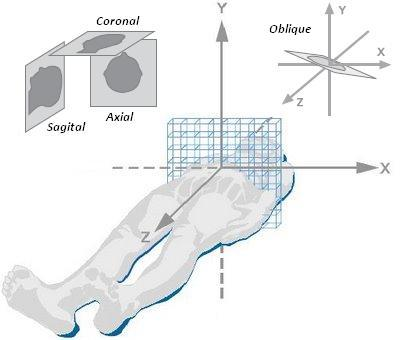
\includegraphics[scale=0.8]{Images/2_axes2.jpg}
	\caption{\textsc{mri} axis planes [sic]: coronal, sagittal and axial.}
	\small Image taken from \cite{Bean2014}.
	\label{svd-axes}
\end{figure}

As shown in Figure \ref{svd-term-fig}, \textit{volume} refers to a three-dimensional region of the scan, a \textit{point} is a single voxel in the volume, and a \textit{slice} is a cross-sectional image taken from the volume. Axial slices are taken by fixing the $z$ coordinate. Note that \textit{lines} will not be used in this thesis.

\begin{figure}[ht]
	\centering
	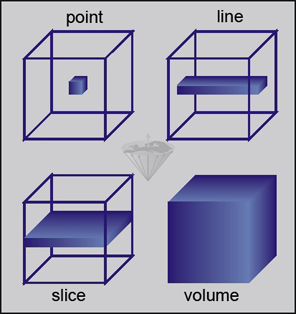
\includegraphics[scale=0.6]{Images/2_mri_volumes.jpg}
	\caption{\textsc{mri} volumes: point, line, slice and volume}
	\small Image taken from \cite{Rinck2013}.
	\label{svd-term-fig}
\end{figure}

Directional terminology in \textsc{mri} include:
\begin{itemize}
	\item \textit{anterior} and \textit{posterior}, referring to objects situated towards the front and back of the body respectively;
	\item \textit{superior} and \textit{inferior}, referring to objects situated above and below other parts of the body respectively; and
	\item \textit{interior} and \textit{exterior}, referring to objects situated closer to and further from the $x=0$ sagittal plane respectively.
\end{itemize}

\subsection*{Structure of the brain}\label{svd-brain}

% Cerebrum diagram
\begin{figure}[ht]
	\centering
	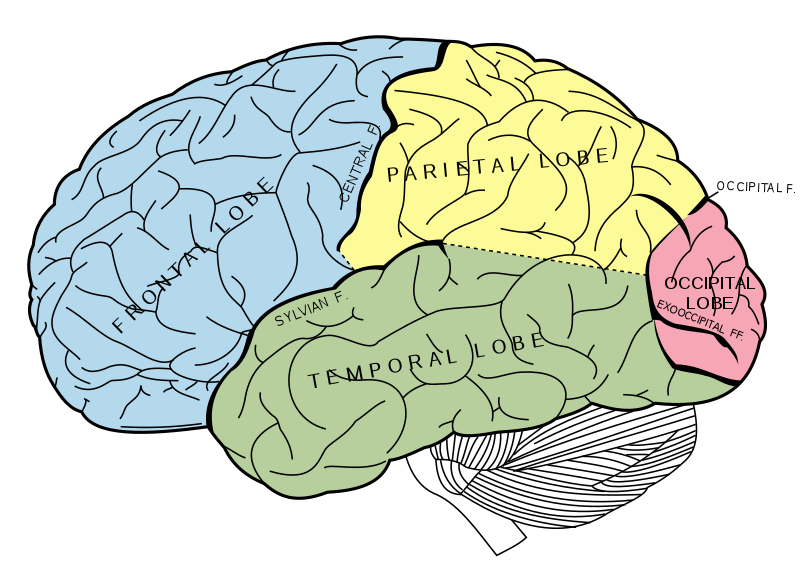
\includegraphics[width=0.7\textwidth]{Images/2_Lobes_of_the_brain_NL.png}
	\caption{The four lobes of the cerebral cortex.}
	\small Image taken from Wikimedia Commons: \url{`Gray728.svg'}.
	\label{svd-cerebrumfig}
\end{figure}

Information from throughout the body is communicated via nerves through the spinal cord to the brain. The brain is the most complex organ in the body, tasked with receiving, interpreting, and responding to nerve signals. It can be segmented into a number of regions, each responsible for different roles.

The largest region is the \textit{cerebrum}, shown in Figure \ref{svd-cerebrumfig}, which forms the outer surface of the brain. It is responsible for voluntary actions, senses, thought and memory, and is divided into two hemispheres - left and right. Each hemisphere is divided into four lobes:
 \begin{itemize}
	\item The \textit{frontal lobe}, located at the front of the cerebrum, is responsible for voluntary movement, skills and behaviours, mood, and memory.
	\item The \textit{parietal lobe}, situated posterior to the frontal lobe, is responsible for the senses, including pain, and physical and spatial awareness.
	\item The \textit{temporal lobe}, located exterior to the perietal lobe, is responsible for memory and auditory functions, including hearing and speech.
	\item The \textit{occipital lobe}, located posterior to the parietal lobe, is responsible for visual information.
\end{itemize}

The outer surface of the brain consists of a layer of neurons referred to as \textit{grey matter}. It is here that much of the brain processes occur \cite{Dafny1997}. Underneath the grey matter is a network of fibres that connects the grey matter neurons together. Collectively they form the \textit{white matter}. The grey and white matter are shown in Figure \ref{svd-greywhitefig}.

% Gray vs white matter diagram
\begin{figure}[ht]
	\centering
	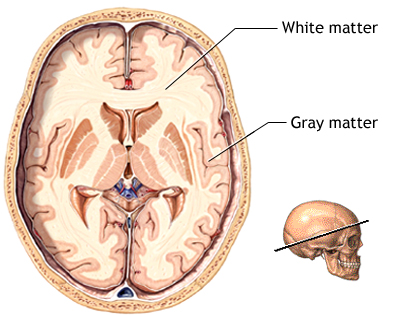
\includegraphics[width=0.6\textwidth]{Images/2_white_vs_grey.png}
	\caption{Grey matter occurs at the surface and within central structures such as the spinal cord. The white matter connects these structures together.}
	\small Image taken from \url{`https://medlineplus.gov/ency/imagepages/18117.htm'}.
	\label{svd-greywhitefig}
\end{figure}

% Basal Ganglia
\begin{figure}[ht]
	\centering
	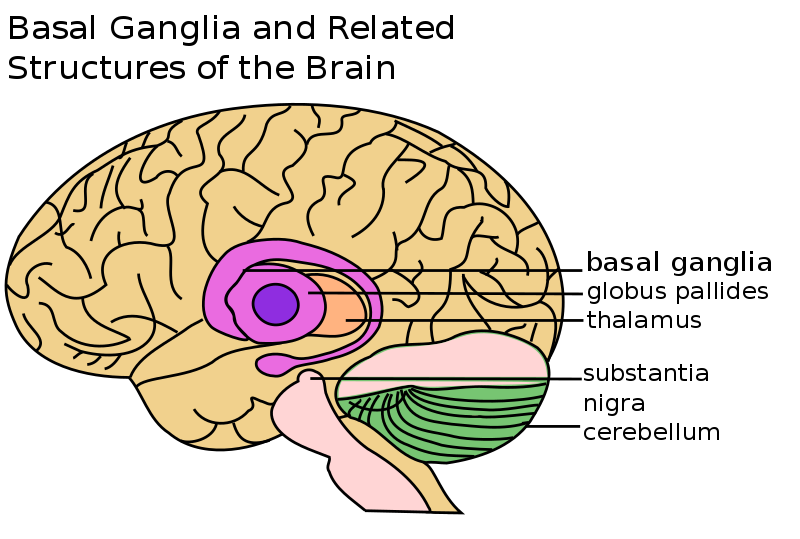
\includegraphics[width=0.7\textwidth]{Images/2_Basal_Ganglia_and_Related_Structures.png}
	\caption{The basal ganglia and other related structures.}
	\small Image taken from Wikimedia Commons: \url{`Basal_Ganglia_and_Related_Structures.svg'}.
	\label{svd-basalfig}
\end{figure}

At the centre of the brain are structures that form the \textit{basal ganglia}, shown in Figure \ref{svd-basalfig}. This region of the brain is responsible for voluntary movement and learning. Connected to this structure is the \textit{thalamus}, which is related to sensory and motor function.
%; and exhibits more numerous instances of lacunes and perivascular spaces. Two structures within the basal ganglia that are often found to have lacunes include the caudate and putamen. The thalamus is another structure that has a high frequency of lacunes, and is interconnected to the basal ganglia.

At the base of the brain lies the \textit{cerebellum}, responsible for coordination; and the \textit{brain stem}, responsible for the transmission of nerve communications. These are shown in Figure \ref{svd-basalfig}. Within the skull, the brain sits in the brain cavity filled with \textit{cerebral spinal fluid} (\textsc{csf}). This fluid can flow between the ridges at the brain's surface, filling gaps throughout the brain matter.


\section{\textsc{mri}}\label{svd-MRI}

\textsc{mri} is a radiological technique that uses magnetic fields and radio waves to generate greyscale images of organs inside the body \cite{Rinck2013}. Three imaging types produced are \textit{T1-weighted}, \textit{T2-weighted} and \textit{FLuid-Attenuated Inversion Recovery} (\textsc{flair}) imaging, shown in Figure \ref{svd-t1-vs-t2}.

% Image comparisons
\begin{figure}[ht]
	\centering
	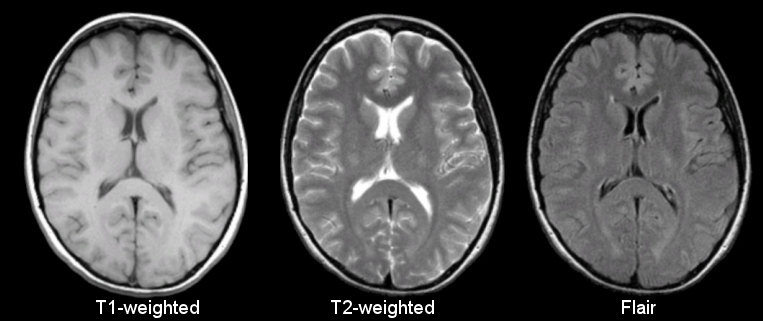
\includegraphics[width=\textwidth]{Images/2_t1_t2_flair.jpg}
	\caption{A comparison of T1, T2 and \textsc{flair} images.}
	\small Image taken from \cite{Preston2006}.
	\label{svd-t1-vs-t2}
\end{figure}

T1-weighted images are \textit{hyperintense} (bright) in regions with high fat content and are \textit{hypointense} (dark) in regions with high water content \cite{Bitar2006}. They therefore return high intensities for brain matter and low intensities for \textsc{csf}. T2-weighted images are hyperintense in regions that contain both high fat and water content \cite{Bitar2006}. This can make it easier to spot abnormalities. \textsc{flair} is an imaging sequence similar to T2-weighted imaging, excepting that \textsc{csf} remains hypointense. Abnormalities will appear bright amongst the darker \textsc{csf}, allowing for easier identification.

\section{\textsc{svd} biomarkers}\label{svd-markers}

During the analysis of \textsc{mri} scans for \textsc{svd}, there are a number of biomarkers that clinicians observe. Each of these is defined in conjunction with the \textsc{strive} criterion \cite{WardlawJ.M.2013Nsfr} shown in Figure \ref{svd-biomarkers-fig}. The schematics show a simplified representation of each biomarker for particular imaging types. Diffusion-weighted imaging (\textsc{dwi}) will not be discussed in this thesis. 

% Images of lacunes and perivascular spaces from \textsc{strive}
\begin{figure}[ht]
	\centering
	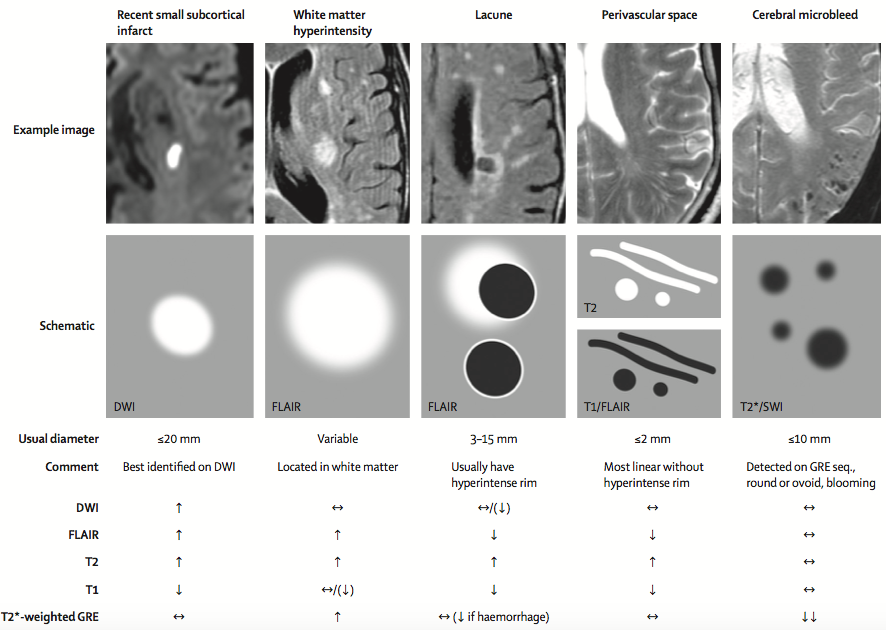
\includegraphics[width = \textwidth]{Images/2_STRIVE.png}
	\caption{\textsc{strive} criterion and \textsc{mri} examples. Up and down arrows indicate hyperintensity and hypointensity respectively. Horizontal arrows indicate structures of the same intensity.}
	\small Image taken from \cite{WardlawJ.M.2013Nsfr}.
	\label{svd-biomarkers-fig}
\end{figure}

\textit{White matter hyperintensities} (\textsc{wmh}) are regions of hyperintensity visible in T2-weighted imaging. They also appear in T1-weighted images as hypointense regions, though not as dark as \textsc{csf}. Their cause is not well understood \cite{Gouw2011}.

\textit{Lacunes} are small brain cavities. They usually appear without symptoms, and are frequently found in the scans of elderly. Their presence indicates a heightened risk of stroke and dementia \cite{BenjaminJ.Philip2018LIbN, VanDerFlierM.Wiesje2005SVDa}. In \textsc{mri}, lacunes appear round, with a diameter between 3 mm and 15 mm. They tend to give off a darker signal intensity, similar to that of \textsc{csf}, as they are filled with fluid. Lacunes have a tendency to occur in regions of white matter hyperintensity, so they will frequently have a hyperintense rim in \textsc{flair} imaging.

\textit{Perivascular spaces} are extensions of the fluid space surrounding blood vessels through the brain. They are generally microscopic but can become enlarged with age, and often appear alongside other \textsc{svd} biomarkers such as lacunes and \textsc{wmh}. Perivascular spaces also take on a signal intensity similar to \textsc{csf} as they are fluid-filled. They are found running parallel to vessels, and are generally found under 3 mm in diameter. They can be identified by appearing circular cross-sectionally and rectangular when viewed in parallel to the vessels. In some instances, perivascular spaces can become enlarged, up to 10 mm in diameter. They can be difficult to distinguish from lacunes as their signal intensities are similar.

\textit{Cerebral microbleeds} are blooming regions of microscopic bleeding, usually around 2--5 mm in diameter though they can be larger. They are not visible on T1-weighted, T2-weighted or \textsc{flair} images, and are instead found in T2*-weighted images constructed from a combination of T2-imaging and inhomogeneities in the magnetic field during scanning. 

\textit{Recent small subcortical infarcts}, are regions of recent oxygen deprivation that have resulted in cell death. They are the cause of 25\% of ischaemic (oxygen starved) strokes \cite{WardlawJ.M.2013Nsfr}. These lesions are usually less than 20 mm in diameter. 

\textit{Brain atrophy} refers to the reduction of brain matter and is not restricted to particular regions of the brain. It can be identified by the increase in \textsc{csf} volume in T1-weighted, T2-weighted and \textsc{flair} imaging.

\section{Image rating}\label{svd-rating}

Without a biopsy for confirmation, the identification of \textsc{svd} biomarkers relies on \textsc{mri} analysis. Trained observers examine \textsc{mri} volumes slice by slice and identify any lesions or points of interest. A number of rating guidelines exist in order to establish rating consistency \cite{AdamsH.H.Hieab2013RMfD, PotterGillian2015CPSV, WardlawJ.M.2013Nsfr}.

Though standardised criterion help to improve rating consistency, the appearance of lacunes and perivascular spaces are highly similar and therefore remain difficult to distinguish. As a result, manual rating is still highly inconsistent \cite{PotterGillian2015CPSV}. Additionally, the manual rating process is time consuming. Heuvel et. al \cite{Heuvel2016} report that the rating of a single scan for microbleeds takes one hour on average. Datasets with many scans can take many hours to process and the resulting identified biomarkers may not be consistent enough to warrant proper inference \cite{BenjaminJ.Philip2018LIbN, WardlawJ.M.2013Nsfr}.

In order to assist clinicians in rating quality, consistency, and speed, machine learning algorithms have been built to identify biomarkers. These algorithms can be built to work either alongside clinicians as computer-aided design (\textsc{cad}) programs \cite{Heuvel2016, Uchiyama20071554, Yokoyama2007} or as fully automated systems \cite{DouQ.2016ADoC, GhafoorianM.2017Dml3}.

%Prior to 2013, there were no official guidelines for the identification of \textsc{svd} biomarkers. There were several studies attempting to establish rating guidelines \cite{AdamsH.H.Hieab2013RMfD, PotterGillian2015CPSV}, however these methods tended to focus on specific events rather than \textsc{svd} biomarkers in general.

%In addition, much of the terminology surrounding some biomarkers was inconsistent. For instance, perivascular spaces are also frequently referred to as Virchow-Robin spaces \cite{AdamsH.H.Hieab2013RMfD, WardlawJ.M.2013Nsfr}.

%In 2013, the \textsc{strive} criterion \cite{WardlawJ.M.2013Nsfr} were established to standardise the terminology and definitions, and visual rating was conducted in conjunction with those guidelines. Though the criterion helped to improve rating consistency, the appearance of lacunes and perivascular spaces are highly similar and therefore remain difficult to distinguish. As a result, manual rating is still highly inconsistent \cite{PotterGillian2015CPSV}. 
%
%In addition, the manual rating process is also time consuming. The checking and logging of an individual scan can take over 10 minutes.

%It is only recently that machine learning algorithms have begun to improve the rating process. Dou et al. \cite{DouQ.2016ADoC} developed a machine learning algorithm for the detection of cerebral microbleeds. This algorithm exhibited a sensitivity of 93.16\%, with an average of 2.74 false positives per slice. 
%
%Ghafoorian et al. \cite{GhafoorianM.2017Dml3} developed a machine learning algorithm for the automated detection of lacunes. This algorithm was able to achieve a sensitivity of 97.4\%, with 0.13 false positives per slice. This algorithm will be discussed further in Section \ref{litrev-ghafoorian}.

%%%%%%%%%%%%%%%%%%%%%%%%%%%%%%%%%%%%%%%%%%%%%%%%%%%%%%%%%%%%%%%%%%%%%%%%%%

%\clearpage

\addcontentsline{toc}{chapter}{References}

\bibliographystyle{apalike}
\bibliography{bibliography.bib}

%\bibliographystyle{apacite}
%\bibliography{mybib.bib}

